\documentclass{article}
\usepackage{tikz}
\begin{document}
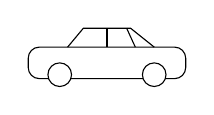
\begin{tikzpicture}
%车底盘
\draw[rounded corners=4pt] (-1,0) rectangle (1,0.4);
%左轮胎
\filldraw[fill=white] (-0.6,0.05) circle (0.15);
%右轮胎
\filldraw[fill=white] (0.6,0.05) circle (0.15);
%车框架
\draw (-0.5,0.4) -- (-0.3,0.64) -- (0.3,0.64) -- (0.6,0.4);
\draw (0,0.4) -- (0,0.64);
\draw (0.25,0.64) -- (0.36,0.4);
\end{tikzpicture}
\end{document}
